\documentclass[12pt]{article}
\setlength\parindent{0pt}
\usepackage{amsmath}
\usepackage{lscape}
\usepackage{graphicx}
\usepackage{fullpage}
\usepackage[margin=0.8in]{geometry}
\setlength{\parskip}{4mm}
\def\LL{\left\langle}   % left angle bracket
\def\RR{\right\rangle}  % right angle bracket
\def\LP{\left(}         % left parenthesis
\def\RP{\right)}        % right parenthesis
\def\LB{\left\{}        % left curly bracket
\def\RB{\right\}}       % right curly bracket
\def\PAR#1#2{ {{\partial #1}\over{\partial #2}} }
\def\PARTWO#1#2{ {{\partial^2 #1}\over{\partial #2}^2} }
\def\PARTWOMIX#1#2#3{ {{\partial^2 #1}\over{\partial #2 \partial #3}} }
\newcommand{\BE}{\begin{displaymath}}
\newcommand{\EE}{\end{displaymath}}
\newcommand{\BNE}{\begin{equation}}
\newcommand{\ENE}{\end{equation}}
\newcommand{\BEA}{\begin{eqnarray}}
\newcommand{\EEA}{\nonumber\end{eqnarray}}
\newcommand{\EL}{\nonumber\\}
\newcommand{\la}[1]{\label{#1}}
\newcommand{\ie}{{\em i.e.\ }}
\newcommand{\eg}{{\em e.\,g.\ }}
\newcommand{\cf}{cf.\ }
\newcommand{\etc}{etc.\ }
\newcommand{\Tr}{{\rm tr}}
\newcommand{\etal}{{\it et al.}}
\newcommand{\OL}[1]{\overline{#1}\ } % overline
\newcommand{\OLL}[1]{\overline{\overline{#1}}\ } % double overline
\newcommand{\OON}{\frac{1}{N}} % "one over N"
\newcommand{\OOX}[1]{\frac{1}{#1}} % "one over X"
\pagenumbering{gobble}
\begin{document}
\Large
\centerline{\sc{Tutorial-Exercise -- The Seasons}}

\normalsize

In this exercise, you'll learn what causes the seasons and how they differ in different places on Earth's surface.

Remember that these exercises are not meant for you to do alone; you should work with others near you on them, and should raise your hand and ask questions as you have them.

Your third homework assignment is included on the back of this handout. You should complete it by class time on September 22 and put it in your TA's mailbox.

\section{Things We Know}

People on Earth observe the following about the seasons:

\begin{enumerate}
	\item The Northern Hemisphere has cold temperatures and short days in December, but hot temperatures and long days in June
	
	\item The Southern Hemisphere has hot temperatures and long days in December, but cold temperatures and short days in June
	
	\item These effects are strongest at high latitudes near the poles; they disappear as you get close to the Equator
\end{enumerate}

We also know some things about Earth's orbit. We are not always the same distance from the Sun; to learn why, we'll need to wait for a month. However, we now know the following:

\begin{center}
\begin{tabular}{|c|c|c|}
	\hline
	\null & \bf{July 4} & \bf{January 3} \\ \hline
	{\bf Distance from Earth to Sun} & 152 million km & 147 million km \\ \hline
\end{tabular}
\end{center}

These distances are measured from the Earth's center. Earth is a ball that is around 13,000 km across.

\section{The Changing Distance from the Sun}

We know that the seasons are really caused by the tilt of Earth's axis. But some people believe that the changing seasons are caused by the fact that sometimes we are closer to the Sun and sometimes further away. Since empirical evidence -- {\it what we actually observe} -- is the most important authority in science, you will need to persuade them that this is not true by citing the things above that we observe about the seasons.

Suppose someone says to you: {\it ``I think the seasons are caused by the fact that Earth's orbit is not quite round. We're closer to the Sun sometimes and that makes it hotter; we're further away from the Sun sometimes and that makes it colder.''}

Does this claim agree with the observations above? Working with the people around you, think of as many ways as you can that this claim is {\it inconsistent} with the things we observe on Earth.

\vspace{3in}

\section{Earth's Axial Tilt}

As we've discussed, the seasons are really caused by the tilt of Earth's axis, which is rotated by $23.5^\circ$ with respect to Earth's orbit.

On the next page, you'll find a diagram of Earth on the two solstices, with the directions of the sunlight shown. 

\subsection{Day and Night}

\begin{enumerate}
	\item {Lightly shade the half of Earth currently experiencing nighttime in each diagram, showing us that it is dark there.}
\end{enumerate}	

As the Earth turns, a person standing on our surface will rotate all the way around Earth, traveling along a path of constant latitude. 

For instance, the red stick figure standing on the Tropic of Cancer will travel around Earth along that path in 24 hours.
\begin{enumerate}\addtocounter{enumi}{1}
	
	\item The tall stick figure is at the latitude of Syracuse. Draw in the path that they will travel during one day. (You'll need to do this on both diagrams.)
	
	\item 
	Based on the paths that each stick figure travels along during 24 hours, complete the following. You won't be able to calculate exact numbers -- that's okay! Estimation is fine.
	
\end{enumerate}









\begin{tabular}{|p{50mm}|c|c|}
\hline
	\null & Hours of Sunlight in June & Hours of Sunlight in December \\ \hline
	
	Syracuse (tall stick figure) & & \\[20pt] \hline
	
	Arctic Circle (short, blue) & & \\[20pt] \hline
	
	A person on the Equator & & \\[20pt] \hline
	
	A person in Argentina \newline (draw their path) & & \\[20pt] \hline
\end{tabular}


\section{Location of the Sun at Noon}

The previous work you've done explains the seasons by the changing day length: short days cause winter, while long days cause summer!

However, there's another thing going on, too. We notice that the Sun is lower in the sky in winter and higher in the sky in summer. Can we explain that?

We'll look only at the December solstice diagram here.

For each of the following: 

\begin{enumerate}
	\item Draw a stick figure at the location if there isn't already one there
	
	\item Draw three arrows: one pointing overhead, one pointing to their northern horizon, and one pointing to their southern horizon. Then draw one more arrow: a horizontal arrow pointing at the direction the sunlight is coming from.
	
	\item Determine the position that they would look to see the Sun at noon and label it on your diagram next to the stick figure. Use language like ``High in the northern sky'', ``Low in the southern sky'', ``Directly overhead''.
\end{enumerate}

\begin{itemize}
	\item A person standing on the Arctic Circle
	\item A person in Syracuse
	\item A person standing on the equator
	\item A person standing on the Tropic of Capricorn
\end{itemize}

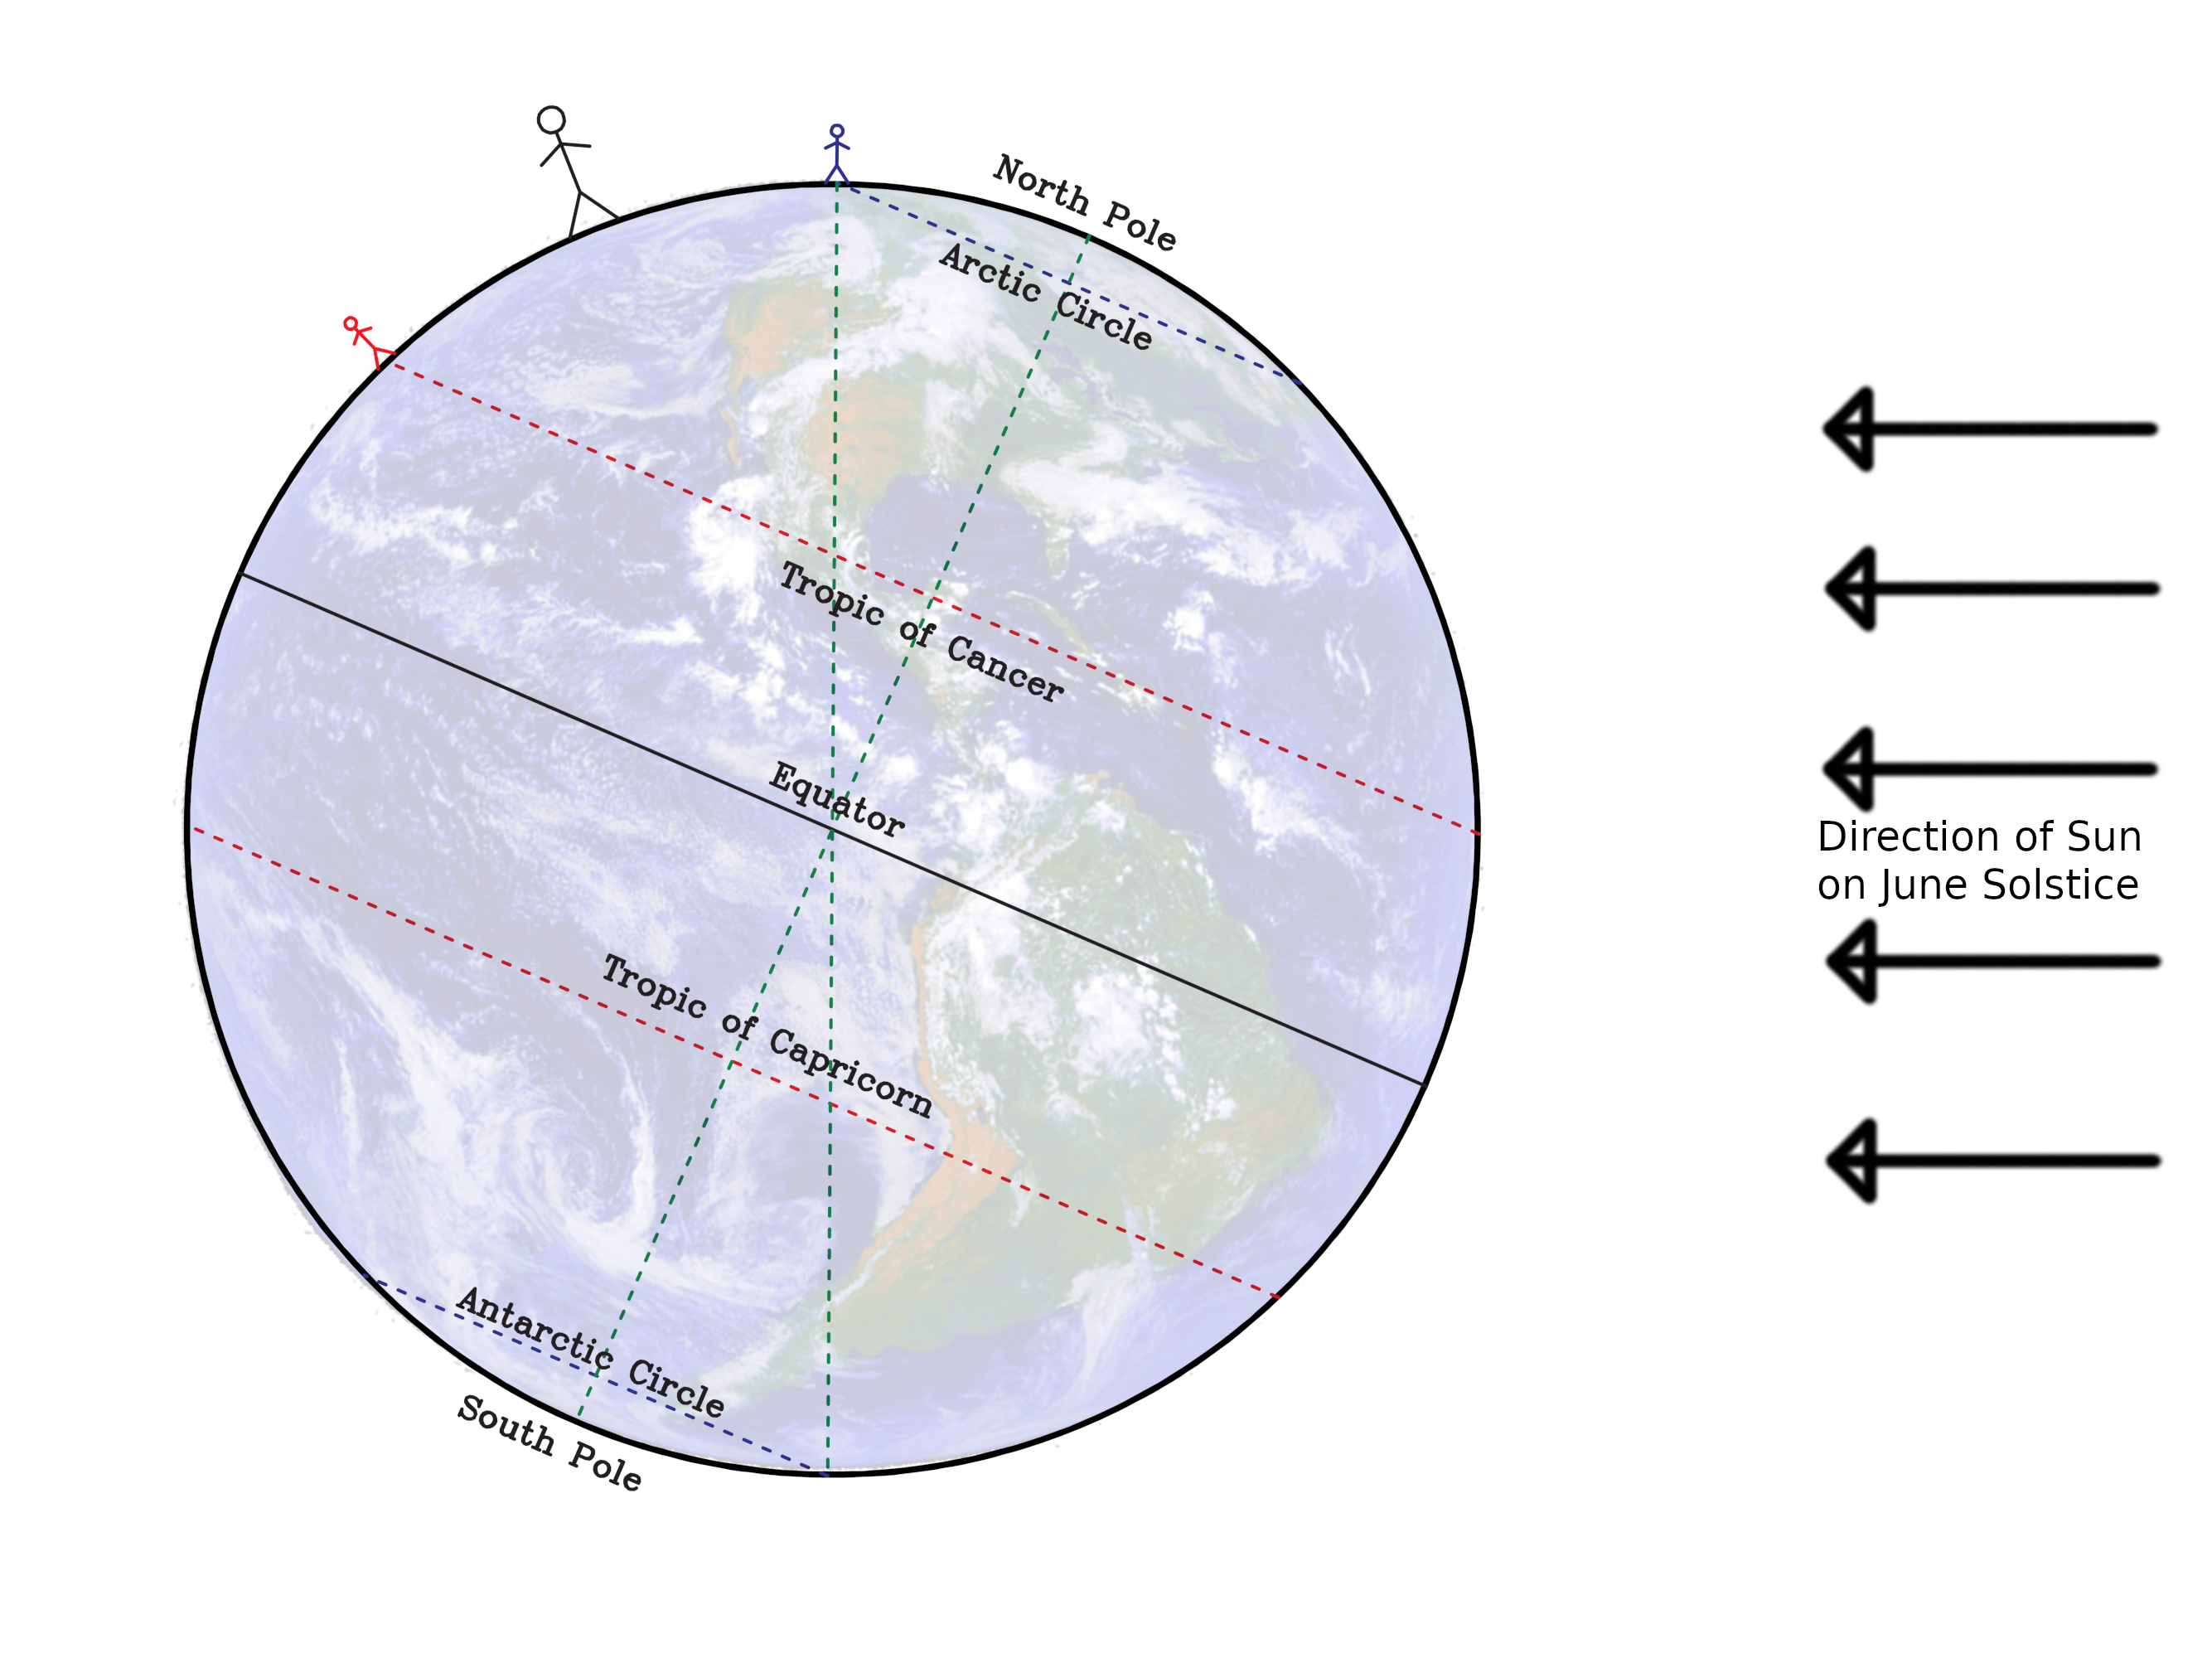
\includegraphics[width=0.85\textwidth]{earth-diagram-june.png}

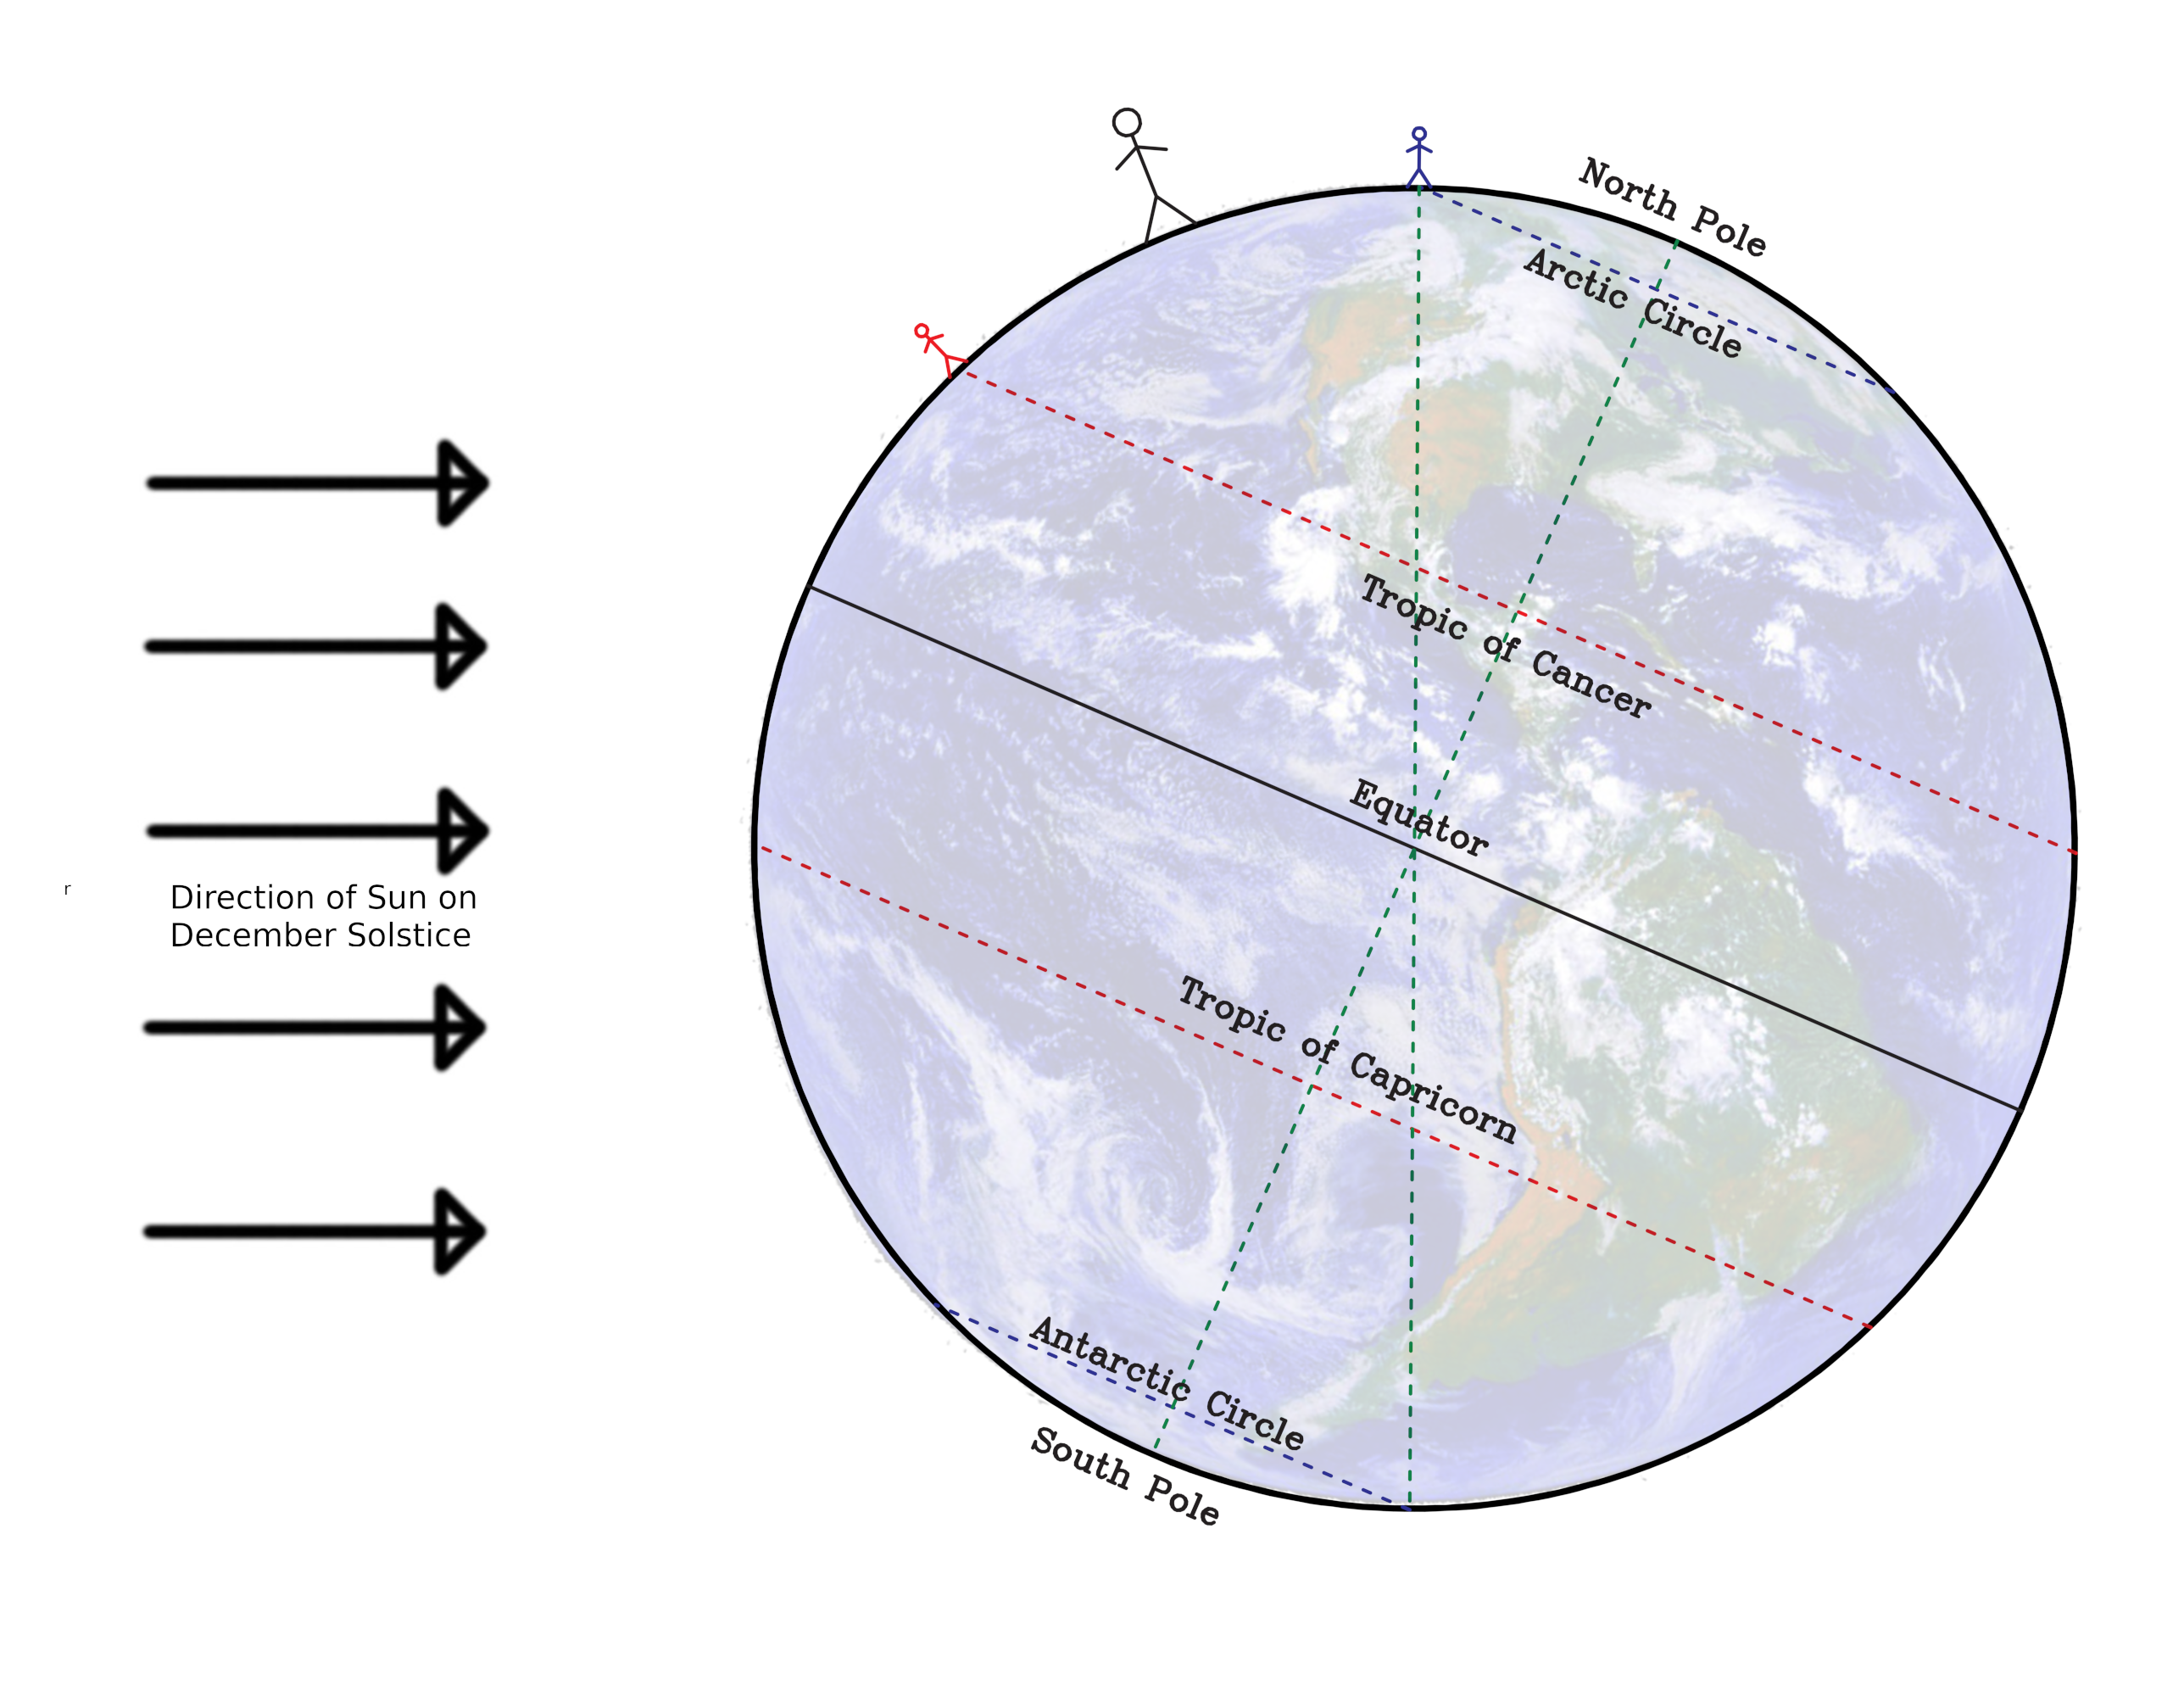
\includegraphics[width=0.85\textwidth]{earth-diagram-december.png}

\newpage

\Large
\centerline{\sc{Homework 3 -- The Seasons}}
\it \begin{center} \normalsize Due to your TA's mailbox by the start of class on Thursday, September 22.\end{center}
\normalsize
\rm

You'll find one large diagram of the Earth on the back of this page, showing both June and December solstices at once. Of course, we know that the Earth travels around the Sun rather than the other way around, but this is a way to use just one diagram to understand everything!

\begin{enumerate}
	\item Label the path that a person in Argentina will take around the Earth as it rotates once. How many hours of sunlight will they have in June? How many hours of sunlight will they have in December?
	
	\vspace{1in}
	
	\item For your person in Argentina, draw a stick figure showing their position at noon in December and in June. (One will be on one side of Earth and the other will be on the other side.)
	
	Where would they look to see the Sun at noon in June? Where would they look to see the Sun at noon in December?
	\vspace{0.8in}	

	\item Where on Earth would a person have to be to see the Sun directly overhead on the June solstice? Draw a stick figure for them.
	\vspace{0.8in}	
	
	\item Where on Earth would a person have to be to never see the Sun at all on the December solstice? Label that location and draw the path that they'll follow as Earth rotates.
		\vspace{0.8in}
		
	\item A person says ``This year I saw the Sun high in the northern sky in June and high in the southern sky in December.'' Where do they live? Draw stick figures for them at noon in June and noon in December.
	
\end{enumerate}

\newpage
\begin{landscape}
	\vspace{1in}
	
	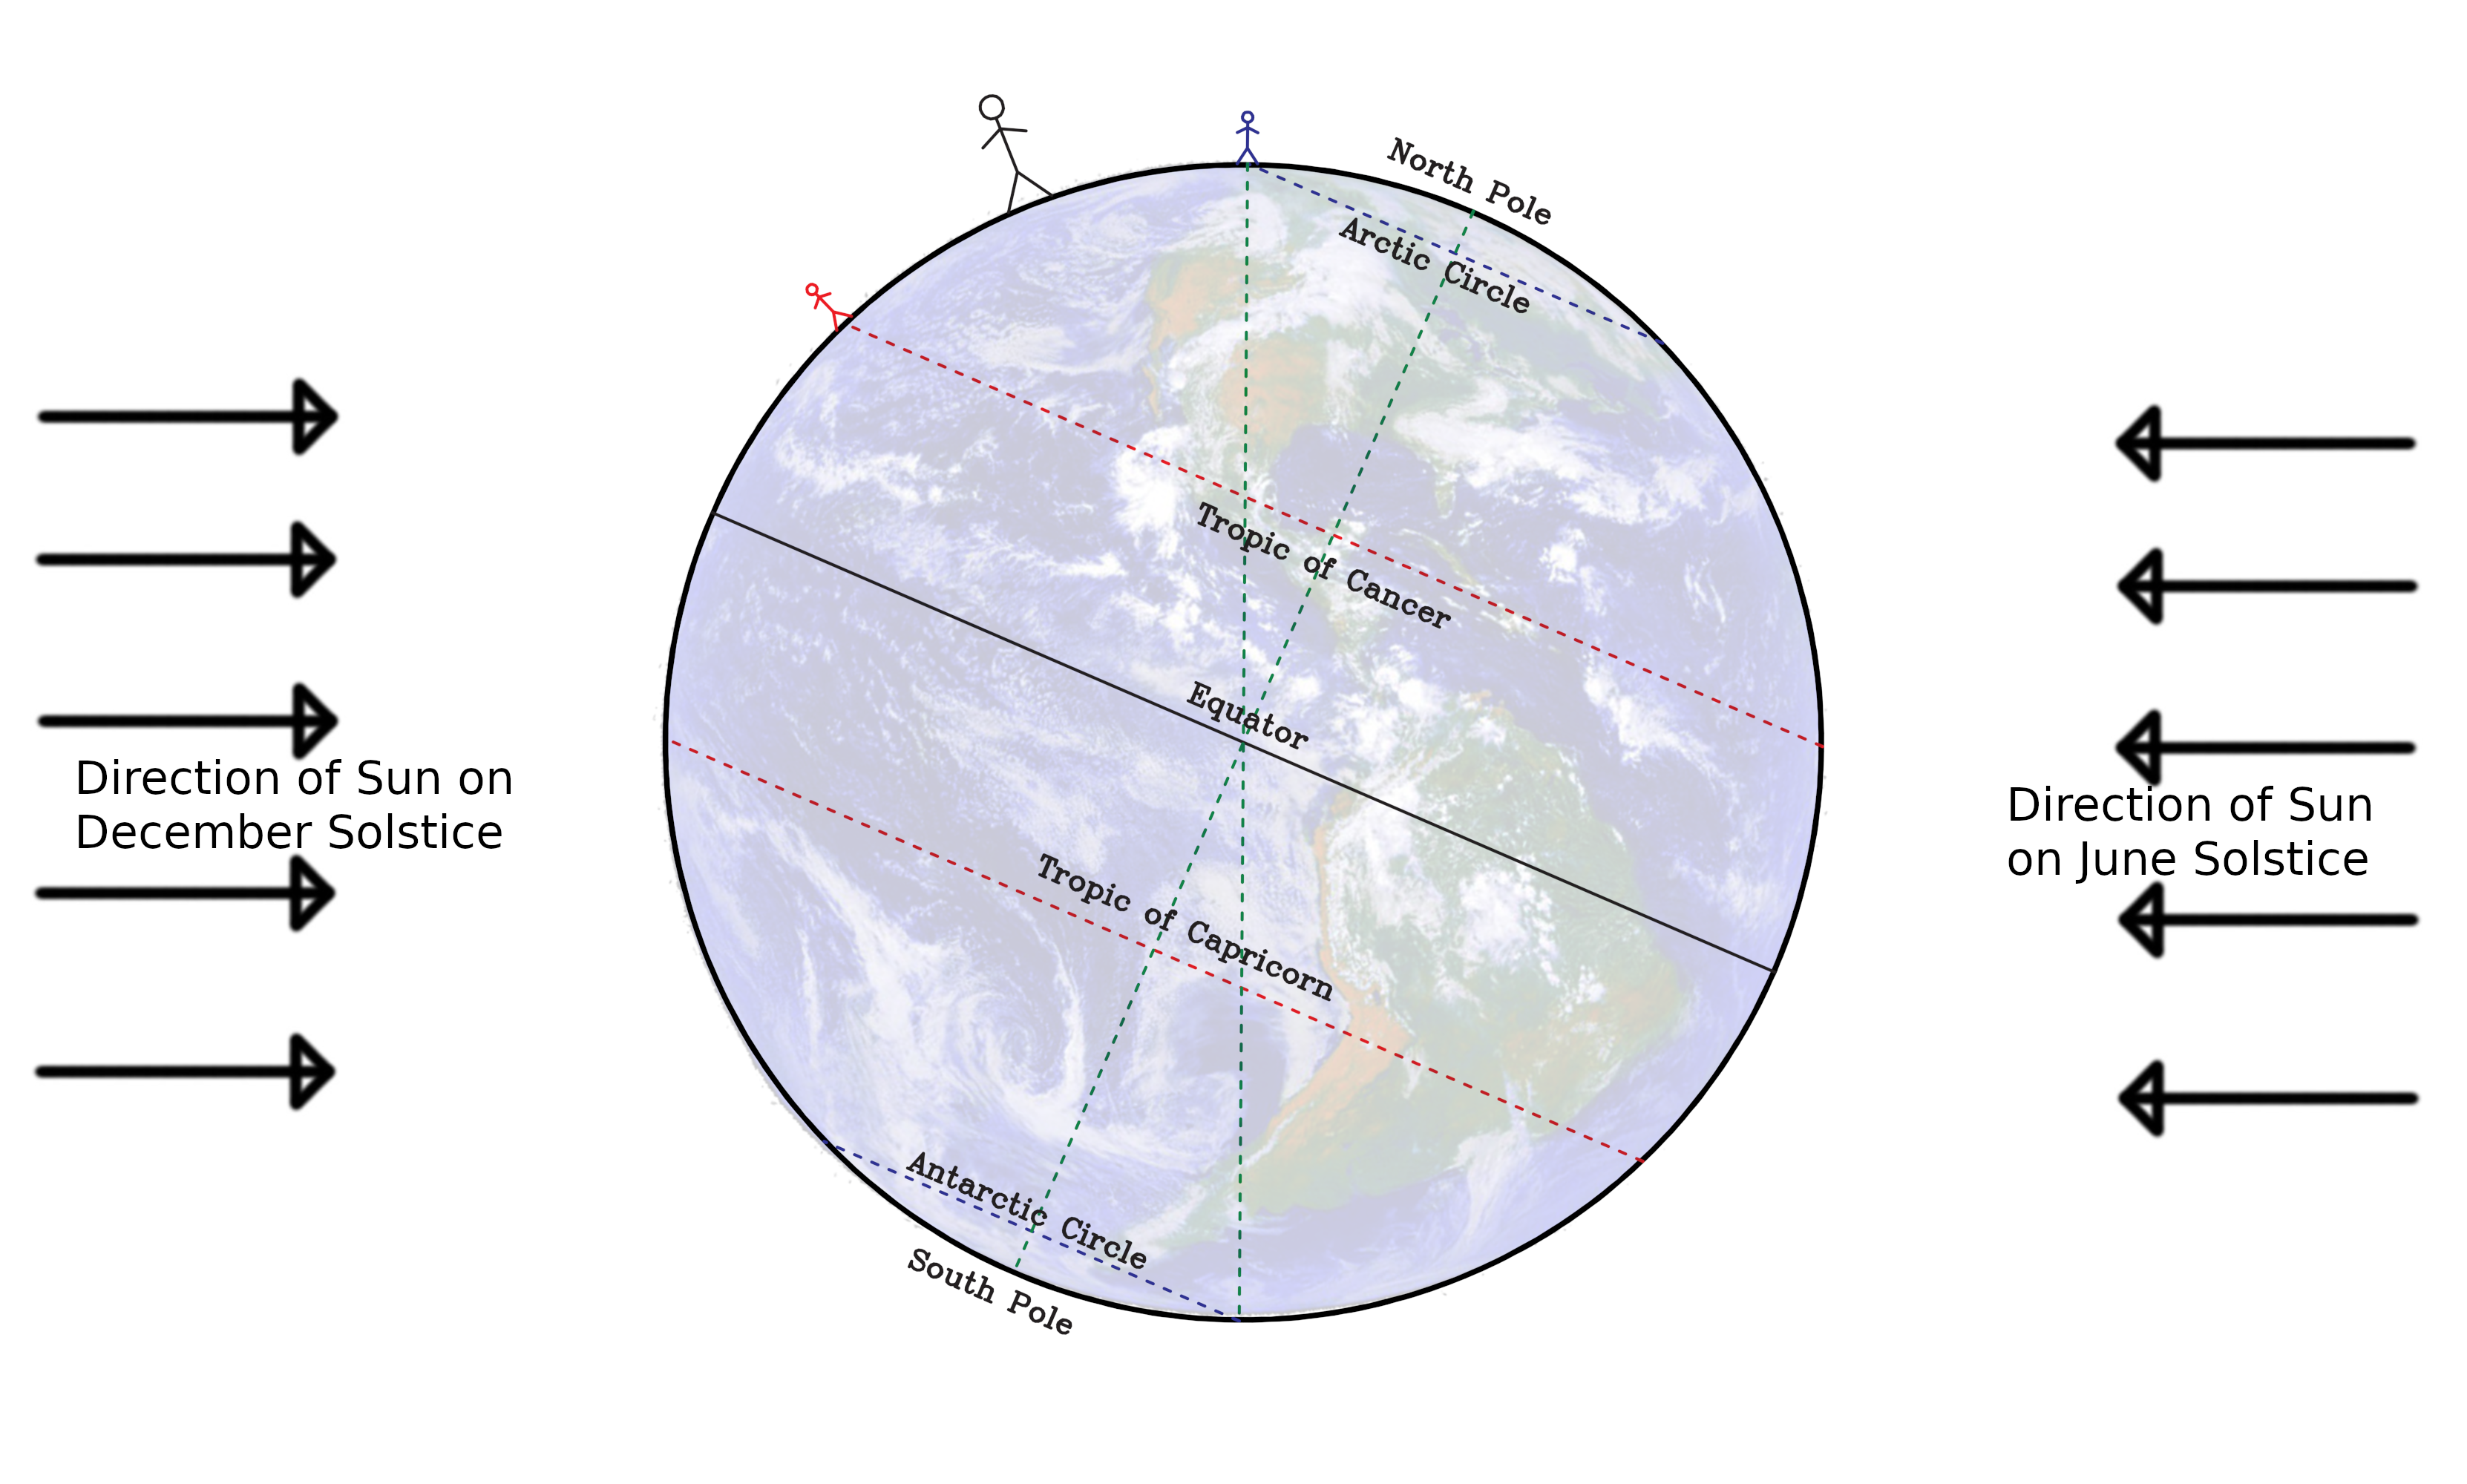
\includegraphics[width=10in]{earth-diagram-both.png}
\end{landscape}

	


\end{document}


